% Created 2020-07-15 mié 08:57
% Intended LaTeX compiler: pdflatex
\documentclass[presentation,aspectratio=169]{beamer}
\usepackage[utf8]{inputenc}
\usepackage[T1]{fontenc}
\usepackage{graphicx}
\usepackage{grffile}
\usepackage{longtable}
\usepackage{wrapfig}
\usepackage{rotating}
\usepackage[normalem]{ulem}
\usepackage{amsmath}
\usepackage{textcomp}
\usepackage{amssymb}
\usepackage{capt-of}
\usepackage{hyperref}
\usepackage{khpreamble}
\usepackage{amssymb}
\DeclareMathOperator{\shift}{q}
\DeclareMathOperator{\diff}{p}
\usetheme{default}
\author{Kjartan Halvorsen}
\date{\today}
\title{Control computarizado - Asignación de polos, parte 2}
\hypersetup{
 pdfauthor={Kjartan Halvorsen},
 pdftitle={Control computarizado - Asignación de polos, parte 2},
 pdfkeywords={},
 pdfsubject={},
 pdfcreator={Emacs 26.3 (Org mode 9.3.6)}, 
 pdflang={English}}
\begin{document}

\maketitle

\section{Conceptos claves - repetición}
\label{sec:orgba70d2b}
\begin{frame}[label={sec:orge66951a}]{Tres conceptos claves}
\begin{enumerate}
\item Dónde poner los polos del sistem en lazo cerrado
\item La función de \emph{sensibilidad} y la función de \emph{sensibilidad complementaria}
\item Determinar el orden del controlador
\end{enumerate}
\end{frame}

\begin{frame}[label={sec:orgb7b7a0f}]{Concepto clave 1) Los polos del sistema en lazo cerrado}
\begin{center}
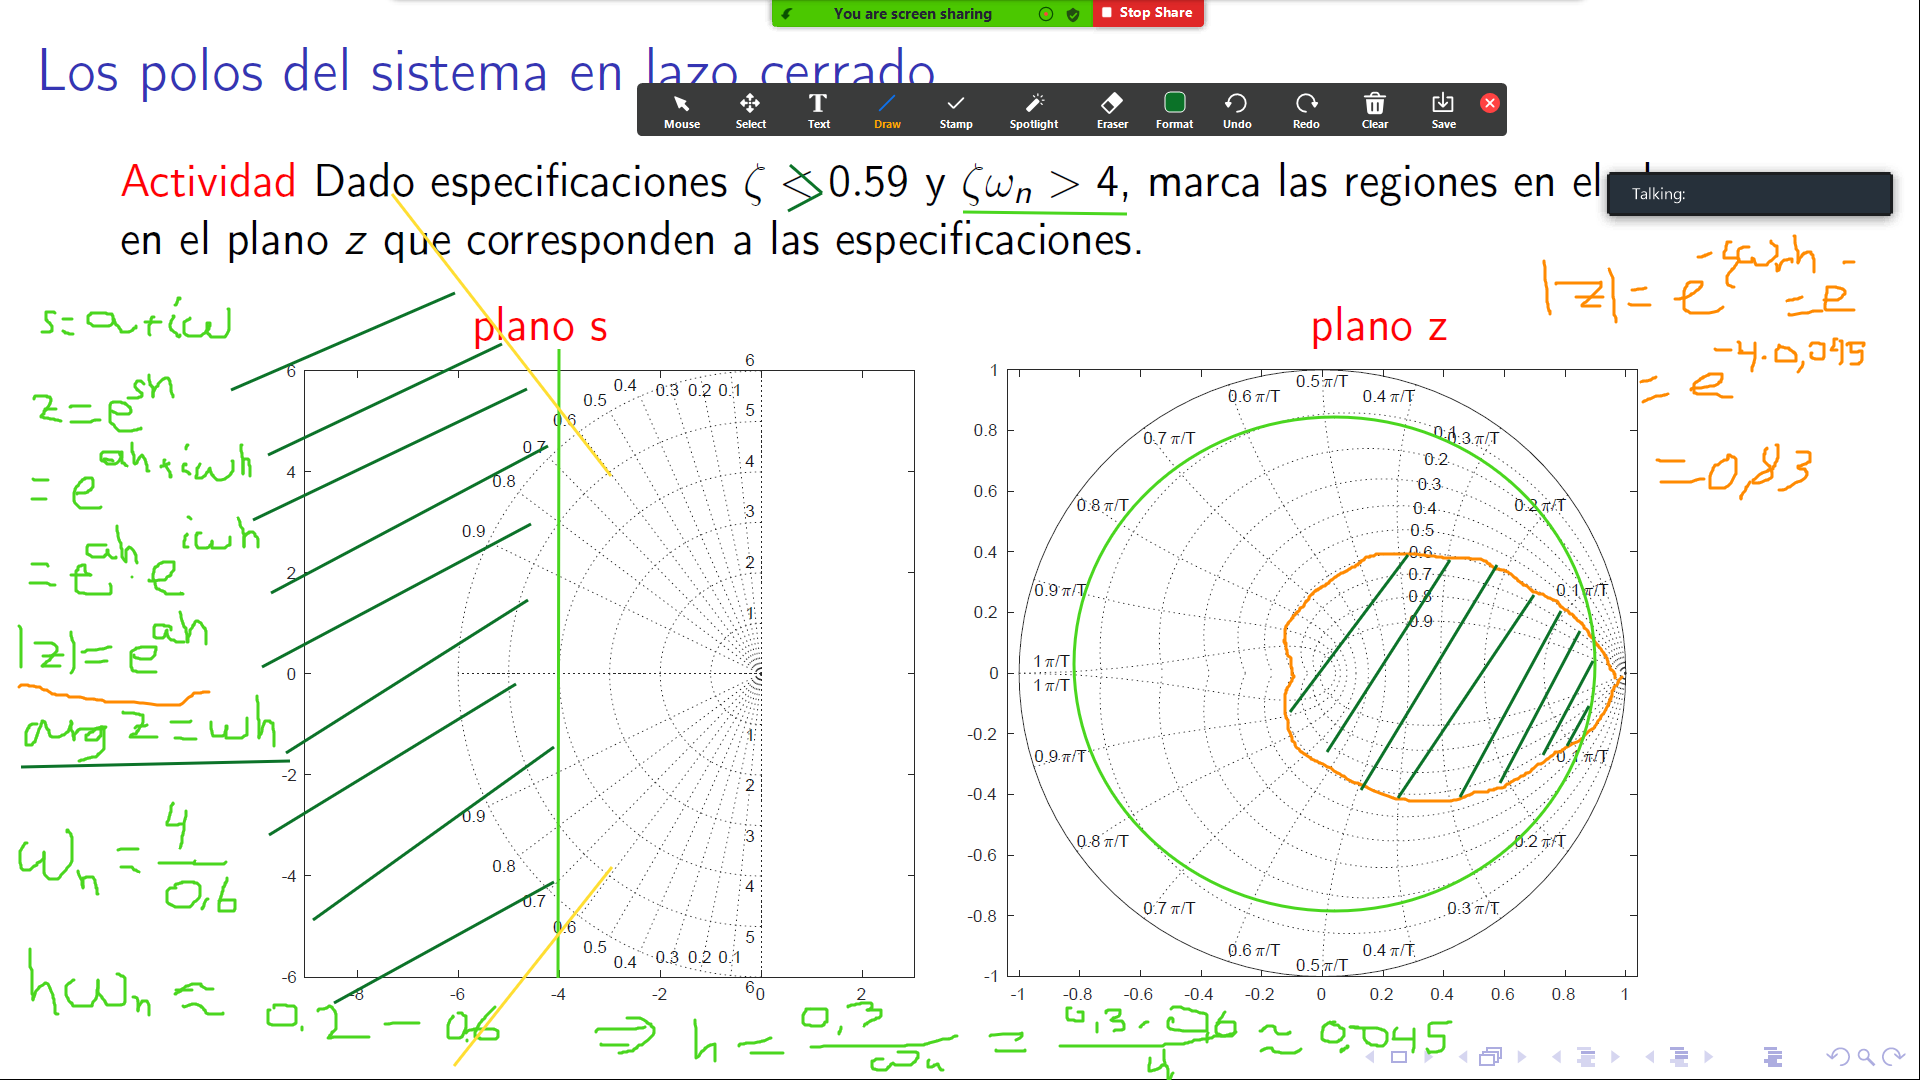
\includegraphics[height=0.8\textheight]{../../figures/screenshot-2020-07-14.png}
\end{center}
\end{frame}

\begin{frame}[label={sec:org0234684}]{Concepto clave 2) Las funciones de sensibilidad y sensibilidad complementaria}
\end{frame}
\begin{frame}[label={sec:org59055cf}]{Controlador de dos grados de libertad}
\begin{center}
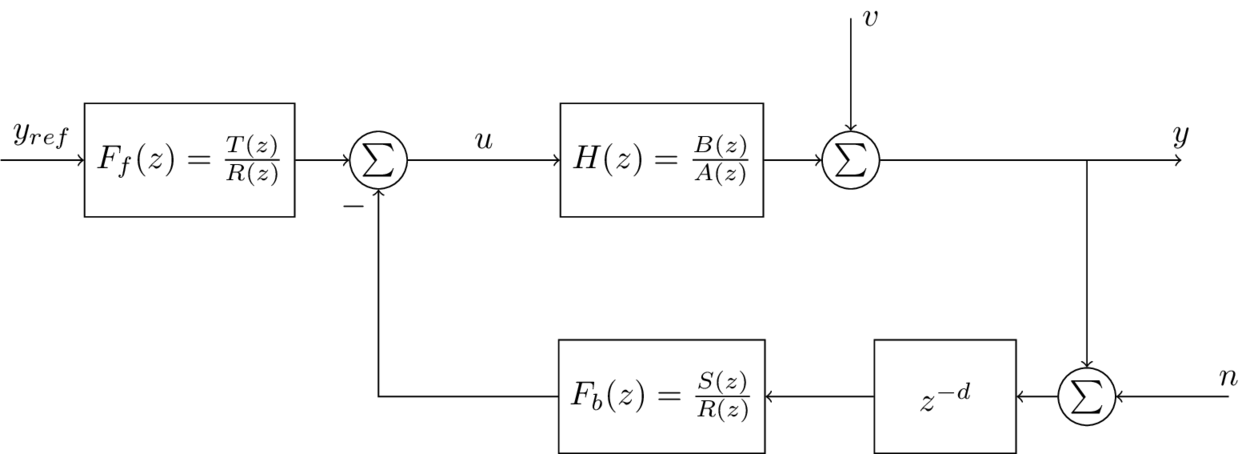
\includegraphics[width=0.7\linewidth]{../../figures/2dof-block-explicit}
\end{center}

\begin{align*}
Y(z)     &= \frac{F_f(z)H(z)}{1 + z^{-d}F_b(z)H(z)}U_c(z) + \overbrace{\frac{1}{1 + z^{-d}F_b(z)H(z)}}^{S_s(z)}V(z)  - \overbrace{\frac{z^{-d}F_b(z)H(z)}{1 + z^{-d}F_b(z)H(z)}}^{T_s(z)}N(z)\\
\end{align*}

\alert{Evidentemente} \(S_s(z) + T_s(z) = 1\) \alert{Conclusion:} Hay que encontrar un equilibrio entre rechazo a perturbaciones y rechazo a ruido de medida.
\end{frame}

\begin{frame}[label={sec:orgdda98ae}]{Sensibilidad y sensibilidad complementaria}
\begin{center}
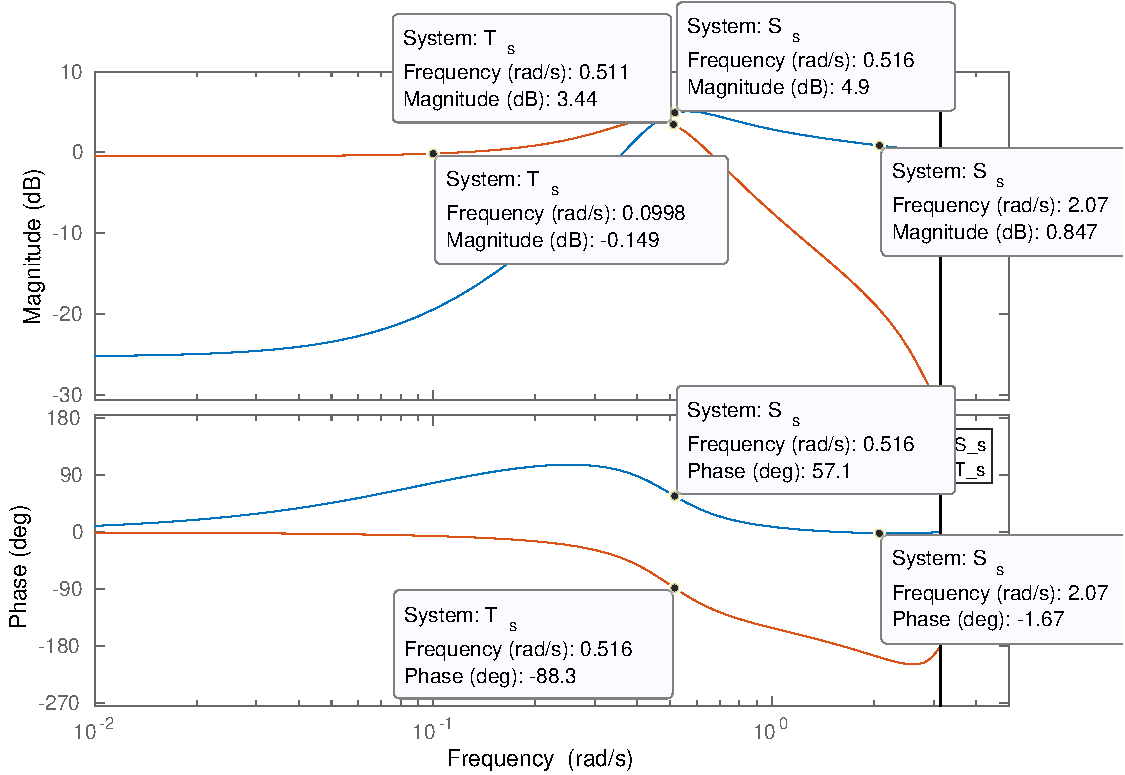
\includegraphics[width=0.7\linewidth]{../matlab/bode-sensitivity-exercise-crop}
\end{center}
\end{frame}


\begin{frame}[label={sec:orgbba2b63}]{Sensibilidad y sensibilidad complementaria -  Solución}
\pgfmathsetmacro{\Smag}{0.12}
\pgfmathsetmacro{\Sarg}{70}
\pgfmathsetmacro{\Tmag}{0.98}
\pgfmathsetmacro{\Targ}{-6}
\pgfmathsetmacro{\Treal}{\Tmag*cos(\Targ)}
\pgfmathsetmacro{\Tim}{\Tmag*sin(\Targ)}

\pgfmathsetmacro{\Smagtwo}{0.12}
\pgfmathsetmacro{\Sargtwo}{70}
\pgfmathsetmacro{\Srealtwo}{\Smagtwo*cos(\Sargtwo)}
\pgfmathsetmacro{\Simtwo}{\Smag*sin(\Sarg)}
\pgfmathsetmacro{\Tmagtwo}{0.98}
\pgfmathsetmacro{\Targtwo}{-6}

\begin{center}
  \begin{tikzpicture}[scale=1.6]

    \draw[->] (-2, 0) -- (2, 0) node[below] {Re};
    \draw[->] (0,-2) -- (0,2) node[left] {Im};
    \draw (1,0) -- (1,-0.05) node[below] {1};
    \draw (-1,0) -- (-1,-0.05) node[below] {-1};
    \draw (0,1) -- (-0.05,1) node[left] {i};
    \draw (0,-1) -- (-0.05,-1) node[left] {-i};
 

    \foreach \Tmag/\Targ/\nn in {-0.149/-6/1, 3.44/-88/2, -19/-196/3} {
       \pgfmathsetmacro{\Treal}{pow(10,\Tmag/20)*cos(\Targ)}
       \pgfmathsetmacro{\Tim}{pow(10,\Tmag/20)*sin(\Targ)}
       \node[circle, fill, orange, inner sep= 1pt] (Tone) at (\Treal, \Tim) {};
           \draw[thin, ->, orange] (0,0) to (Tone) node[right] {\tiny \nn};
	   }
    \foreach \Smag/\Sarg/\nn in {-18/78/1, 4.9/57/2, 0.85/-1.67/3} {
       \pgfmathsetmacro{\Sreal}{pow(10,\Smag/20)*cos(\Sarg)}
       \pgfmathsetmacro{\Sim}{pow(10,\Smag/20)*sin(\Sarg)}
       \node[circle, fill, blue!80, inner sep= 1pt] (Sone) at (\Sreal, \Sim) {};
           \draw[thin, ->, blue!80] (0,0) to (Sone) node[right] {\tiny \nn};
	   }

    %\node[circle, fill, blue!80, inner sep= 1pt] (Sone) at (\Sreal, \Sim) {};
    %\draw[thin, ->, blue!80] (0,0) to (Sone);
  \end{tikzpicture}
\end{center}
\end{frame}


\begin{frame}[label={sec:orgcb5978e}]{La función de sensibilidad}
\[S_s(z) = \frac{1}{1 + z^{-d}F_b(z)H(z)} = \frac{1}{1 + G_o(z)}= \frac{1}{G_o(z) - (-1)}\]


\begin{columns}
\begin{column}{0.45\columnwidth}
\[|S_s(\mathrm{e}^{i\omega h})| = |S_s(i\omega)| = \frac{1}{| G_o(i\omega) - (-1)|}\]

\alert{La magntiúd de la función de sensibilidad es inversa proporcional  a la distancia de la curva de Nyquist al punto critico -1}
\end{column}

\begin{column}{0.65\columnwidth}
\begin{center}
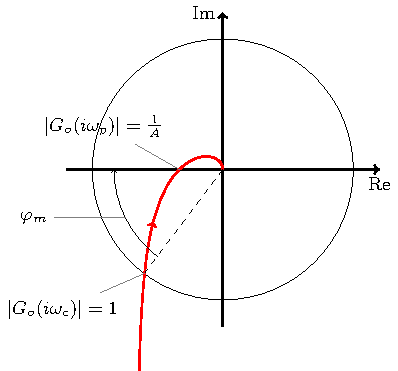
\includegraphics[width=0.6\linewidth]{../../figures/implane-nyquist-margins}
\end{center}
\end{column}
\end{columns}
\end{frame}

\begin{frame}[label={sec:org6533b94}]{La función de sensibilidad - ejercicio}
\alert{Actividad} Dibuja la magnitúd de la funcion de sensibilidad, dado la curva de Nyquist.

\begin{columns}
\begin{column}{0.65\columnwidth}
    \begin{center}
    \begin{tikzpicture}
  \begin{loglogaxis} [
      clip=false,
      ylabel=$|S_s(i\omega)|$,
      width=9cm,
      height=5cm,
      %grid=both,
      ytick={0.1, 1, 10},
      xticklabel=\empty,
      ymin=0.1, ymax=10,
      xmin=0.1, xmax=10,
      every major grid/.style={red, opacity=0.5},
      %legend entries={Bessel filter, Delay of one},
      %legend pos={south west},
  ]
 %   \addplot 
 %   shell[thick,black, no marks, prefix=pgfshell_, id=bodenm,] {julia -q --eval  "G=tf([3],[(1.0/\omegazero)^2, 3/\omegazero, 3]); print_bode_phase(G, -2, 2);"};
 \draw[orange!90!black] (axis cs: 1, 0.13) -- (axis cs: 1, 0.1) node[below] {$\omega_c$};
 \draw[orange!90!black] (axis cs: 3, 0.13) -- (axis cs: 3, 0.1) node[below] {$\omega_p$};
  \end{loglogaxis}
\end{tikzpicture}
\end{center}
\end{column}


\begin{column}{0.35\columnwidth}
\begin{center}
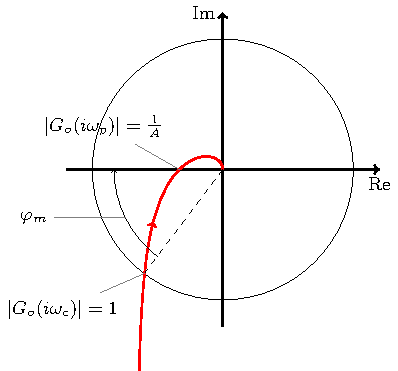
\includegraphics[width=0.99\linewidth]{../../figures/implane-nyquist-margins}
\end{center}
\end{column}
\end{columns}
\end{frame}


\section{Cancelación de polos del observador}
\label{sec:org08f309c}
\begin{frame}[label={sec:org83498a8}]{Controlador de dos grados de libertad}
\begin{center}
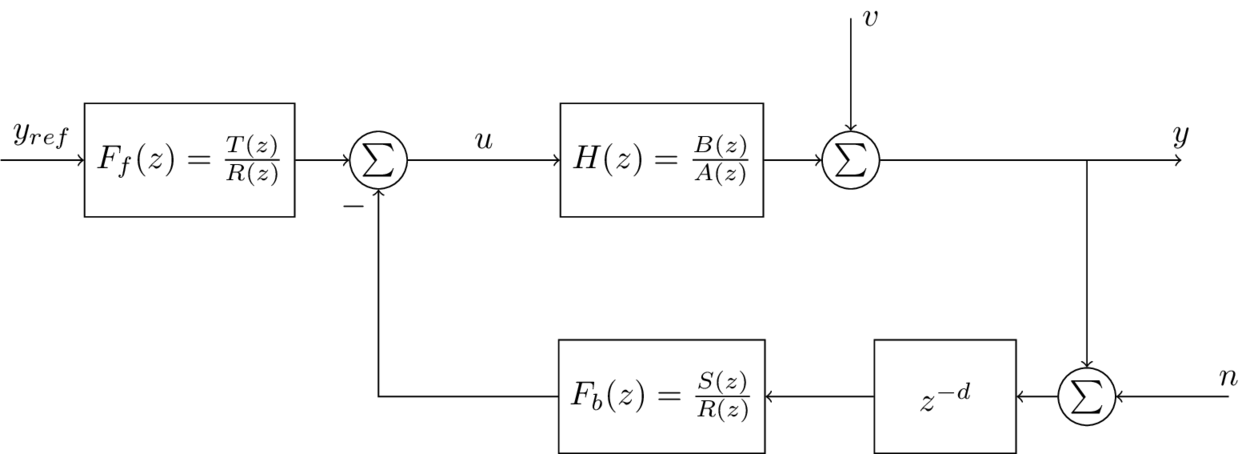
\includegraphics[width=0.7\linewidth]{../../figures/2dof-block-explicit}
\end{center}

\begin{align*}
Y(z) &= \frac{T(z)B(z)z^d}{z^dA(z)R(z) + B(z)S(z)}U_c(z) + \frac{A(z)R(z)z^d}{z^dA(z)R(z) + B(z)S(z)}V(z)\\ & \qquad\qquad\qquad - \frac{S(z)B(z)}{z^dA(z)R(z) + B(z)S(z)}N(z)
\end{align*}
\end{frame}

\begin{frame}[label={sec:orgde00223}]{Controlador de dos grados de libertad}
\begin{center}
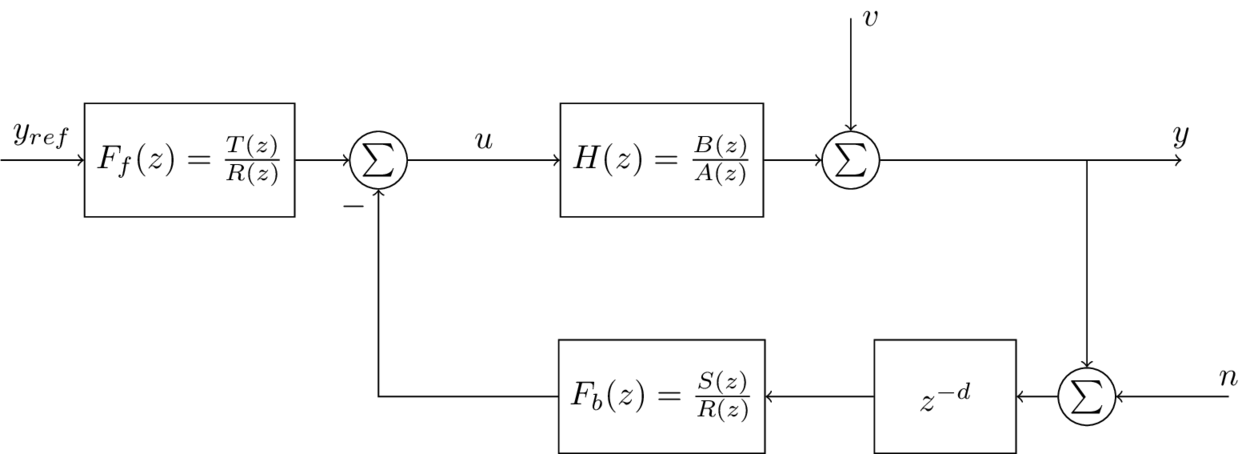
\includegraphics[width=0.7\linewidth]{../../figures/2dof-block-explicit}
\end{center}
\begin{align*}
Y(z) &= \frac{t_0B(z)z^d}{A_c(z)}U_c(z) + \frac{A(z)R(z)z^d}{A_c(z)A_o(z)}V(z)- \frac{S(z)B(z)}{A_c(z)A_o(z)}N(z)
\end{align*}
\alert{Conclusiones} 1) Hay una separación parcial entre seguimiento de la referencia y rechazo a perturbaciones. 2) Se puede usar los polos correspondientes a las raíces de \(A_o(z)\) para afinar el rechazo a perturbaciones contra rechazo a ruido de medida. 
\end{frame}


\section{RST}
\label{sec:orga0d15e5}

\begin{frame}[label={sec:orgc9b04c4}]{Procedimiento - asignación de polos}
Dado modelo del proceso \(H(z)=\frac{B(z)}{A(z)}\), y especificaciones de polos deseados del sistema en lazo cerrado \(A_{cl}(z) = (z-\alpha_1)(z-\alpha_2) \cdots (z-\alpha_{n_c})\)
\begin{enumerate}
\item Determina la ecuación diofantina
\[ A(z)R(z)z^{d} + B(z)S(z) = A_{cl}(z) \]
y el orden adecuado del controlador, con \(\deg S = \deg R\).
\item Factoriza el polinomio caracteristico del lazo cerrado \(A_{cl}(z) = A_c(z)A_o(z)\), donde \(n_{A_o} = n_R\).
\item Determina polinomios \(R(z)\) y \(S(z)\) que satisfican
\[ A(z)R(z)z^{d} + B(z)S(z) = A_{cl}(z) \]
\end{enumerate}
\end{frame}

\begin{frame}[label={sec:org20bd6cf}]{Procedimiento}
Dado modelo del proceso \(H(z)=\frac{B(z)}{A(z)}\), y especificaciones de polos deseados del sistema en lazo cerrado \(A_{cl}(z) = (z-\alpha_1)(z-\alpha_2) \cdots (z-\alpha_{n_c})\)
\begin{enumerate}
\setcounter{enumi}{3}
\item Elige
\[T(z) = t_0 A_o(z),\] donde \(t_0 = \frac{A_c(1)}{B(1)}\).
\end{enumerate}

Obtenemos la \alert{ley de control} 
\[ R(q) u(k) = T(q)u_c(k) - S(q)y(k). \]
y la respuesta en lazo cerrado a la señal de referencia
\[ y(k) = \frac{t_0 B(q)}{A_c(q)} u_c(k). \]
\end{frame}

\begin{frame}[label={sec:orgd1ca991}]{Concepto clave 3) Determinando el orden del controlador}
Tenemos la ecuación diofantina
   \[ A(z)R(z)z^{d} + B(z)S(z) = A_{cl}(z) \qquad (*) \]
y el controlador
\[F_b(z) = \frac{S(z)}{R(z)} = \frac{s_0z^n + s_1z^{n-1} + \cdots + s_n}{z^n + r_1 z^{n-1} + \cdots + r_n}\]
\alert{¿Cómo decidir el orden del controlador?} Nota
\begin{itemize}
\item el controlador tiene \(n+n+1 = 2\deg R + 1\) parámetros desconocidos
\item el lado izquierdo de \((*)\) tiene el grado \(\deg \big(A(z)R(z)z^d + B(z)S(z)\big) = \deg A + \deg R + d\)
\item la ecuación diofantina da un numero de ecuaciones (no-triviales) igual a su grado, al poner iguales los coeficientes correspondientes de los dos lados.

\alert{\(\Rightarrow\;\)Elige \(\deg R\) que satisface \(2\deg R + 1 = \deg A + \deg R + d\)}
\end{itemize}
\end{frame}


\section{Ejemplo}
\label{sec:org14410bd}
\begin{frame}[label={sec:orgc5d90c9}]{Ejemplo - Control de nivel de una presa}
\begin{center}
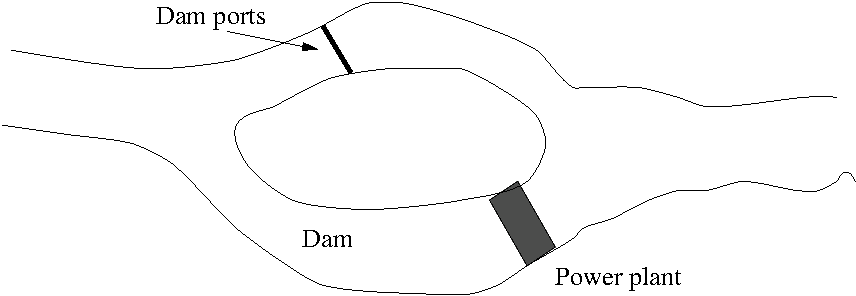
\includegraphics[width=0.5\linewidth]{../../figures/kraftverk}
\end{center}

\alert{Objetivo} Obtener un sistema en lazo cerrado con polos en \(z=0.9\).
\end{frame}

\begin{frame}[label={sec:org150d10b}]{Ejemplo - Control de nivel de una presa}
\begin{center}
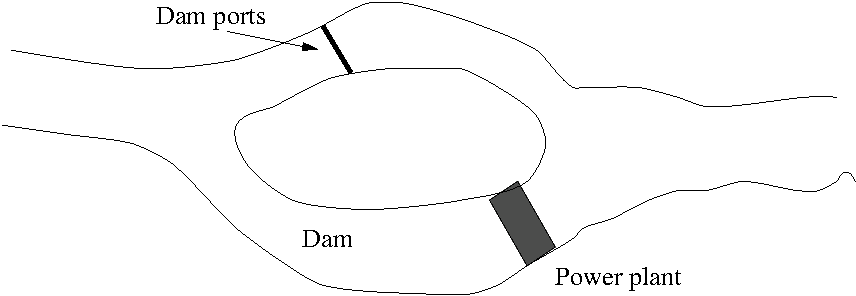
\includegraphics[width=0.3\linewidth]{../../figures/kraftverk}
\end{center}

\alert{Dinámica del proceso}

\begin{center}
  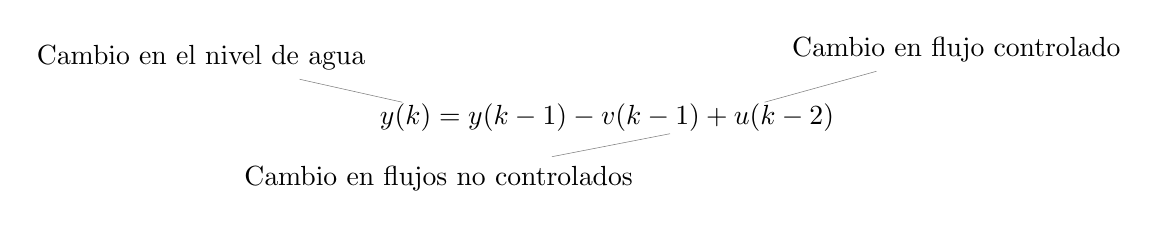
\begin{tikzpicture}
    \node at (0,0) {$y(k) = y(k-1) -v(k-1) + u(k-2)$};
    \node[coordinate, pin=140:{Cambio en el nivel de agua}] at (-2.6,0.2) {};
    \node[coordinate, pin=-140:{Cambio en flujos no controlados}] at (0.8,-0.2) {};
    \node[coordinate, pin=60:{Cambio en flujo controlado}] at (2,0.2) {};
\end{tikzpicture}
\end{center}
\begin{center}
  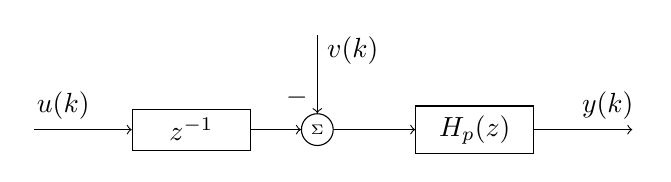
\begin{tikzpicture}[node distance=22mm, block/.style={rectangle, draw, minimum width=15mm}, sumnode/.style={circle, draw, inner sep=2pt}]

    \node[coordinate] (input) {};
    \node[block, right of=input, node distance=20mm] (delay)  {$z^{-1}$};
    \node[sumnode, right of=delay, node distance=16mm] (sum) {\tiny $\Sigma$};
    \node[block, right of=sum, node distance=20mm] (plant)  {$H_p(z)$};
    \node[coordinate, above of=sum, node distance=12mm] (disturbance) {};
    \node[coordinate, right of=plant, node distance=20mm] (output) {};

    \draw[->] (input) -- node[above, pos=0.3] {$u(k)$} (delay);
    \draw[->] (sum) -- node[above] {} (plant);
    \draw[->] (plant) -- node[above, near end] {$y(k)$} (output);
    \draw[->] (disturbance) -- node[right, pos=0.2] {$v(k)$} node[left, pos=0.8] {$-$} (sum);
    \draw[->] (delay) -- (sum);
  \end{tikzpicture}
\end{center}
\end{frame}

\begin{frame}[label={sec:org3ce2375}]{Ejemplo - Control de nivel de una presa}
\alert{Dinámica del proceso}

\begin{center}
  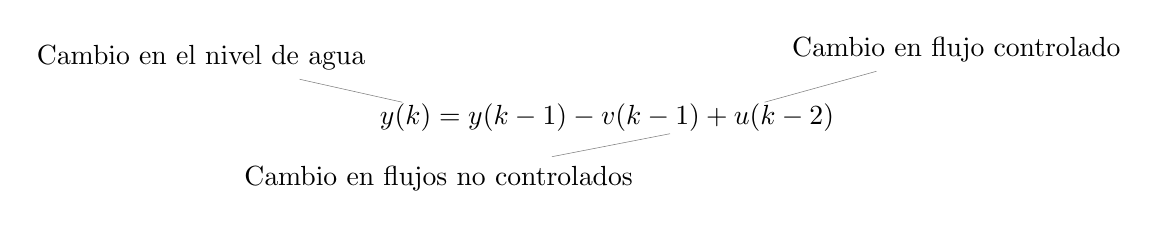
\begin{tikzpicture}
    \node at (0,0) {$y(k) = y(k-1) -v(k-1) + u(k-2)$};
    \node[coordinate, pin=140:{Cambio en el nivel de agua}] at (-2.6,0.2) {};
    \node[coordinate, pin=-140:{Cambio en flujos no controlados}] at (0.8,-0.2) {};
    \node[coordinate, pin=60:{Cambio en flujo controlado}] at (2,0.2) {};
\end{tikzpicture}
\end{center}
\begin{center}
  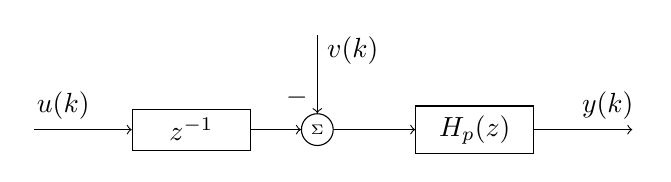
\begin{tikzpicture}[node distance=22mm, block/.style={rectangle, draw, minimum width=15mm}, sumnode/.style={circle, draw, inner sep=2pt}]

    \node[coordinate] (input) {};
    \node[block, right of=input, node distance=20mm] (delay)  {$z^{-1}$};
    \node[sumnode, right of=delay, node distance=16mm] (sum) {\tiny $\Sigma$};
    \node[block, right of=sum, node distance=20mm] (plant)  {$H_p(z)$};
    \node[coordinate, above of=sum, node distance=12mm] (disturbance) {};
    \node[coordinate, right of=plant, node distance=20mm] (output) {};

    \draw[->] (input) -- node[above, pos=0.3] {$u(k)$} (delay);
    \draw[->] (sum) -- node[above] {} (plant);
    \draw[->] (plant) -- node[above, near end] {$y(k)$} (output);
    \draw[->] (disturbance) -- node[right, pos=0.2] {$v(k)$} node[left, pos=0.8] {$-$} (sum);
    \draw[->] (delay) -- (sum);
  \end{tikzpicture}
\end{center}
\alert{Actividad} ¿Cuál es la funcion de transferencia de \(u(k)\) a \(y(k)\)?

\begin{center}
\begin{tabular}{lll}
1: \(H(z) = \frac{z}{z-1}\) & 2: \(H(z)=\frac{1}{z-1}\) & 3: \(H(z)=\frac{1}{z(z-1)}\)\\
\end{tabular}
\end{center}
\end{frame}


\begin{frame}[label={sec:org8065e55}]{Ejemplo - Control de nivel de una presa}
Dado proceso \(H(z) = \frac{B(z)}{A(z)} = \frac{1}{z(z-1)}\) y polos deseados en \(z=0.9\).

\begin{enumerate}
\item Ecuación diofantina \(A(z)R(z)z^d + B(z)S(z) = A_{cl}(z)\)
\[ z(z-1)R(z) + S(z) = A_{cl}(z)\]
El orden del controlador es 
\[\deg R = \deg A + d - 1 = 2-1 = 1, \quad \Rightarrow \quad F_b(z)=\frac{S(z)}{R(z)} = \frac{s_0z + s_1}{z + r_1}\]
\item Tenemos la ecuación diofantina
\[ z(z-1)(z+r_1) + s_0z + s_1 = A_{cl}(z)\]
El grado de \(A_{cl}(z)\) es 3. Eligimos \(A_o(z) = z\),  ( \(\deg A_o = \deg R\)) 
\[ A_{cl}(z) = A_o(z) A_c(z) = z(z-0.9)^2\]
\end{enumerate}
\end{frame}

\begin{frame}[label={sec:orgaddd4c3}]{Ejemplo - Control de nivel de una presa}
\begin{enumerate}
\setcounter{enumi}{2}
\item De la ecuación diofantina \[ z(z-1)(z+r_1) + s_0z + s_1 = z(z-0.9)^2\]
\[ z^3 + (r_1-1)z^2 - r_1z + s_0z + s_1 = z^3 -1.8z^2 + 0.81z\]
Obtenemos las ecuaciones 
\begin{align*}
\begin{cases} z^2 &: \quad r_1-1 = -1.8\\
z^1 &: \quad -r_1 + s_0 = 0.81\\
z^0 &: \quad s_1 = 0
\end{cases}
\quad \Rightarrow \quad 
\begin{cases} r_1 &= -0.8\\ s_0 &= 0.01\\ s_1 &=0 \end{cases}
\end{align*}
\[F_b(z) = \frac{0.01z}{z - 0.8}\]
\end{enumerate}
\end{frame}

\begin{frame}[label={sec:org2fafd13}]{Ejemplo - Control de nivel de una presa}
\begin{enumerate}
\setcounter{enumi}{3}
\item Tenemos \(A_o(z) = z\), entonces 
\[T(z) = t_0A_o(z) = t_0z\]
\[G_c(z) = \frac{T(z)B(z)}{A_o(z)A_c(z)} = \frac{t_0 B(z)}{A_c(z)}, \quad \text{queremos}\, G_c(1)=1\]
\[ t_0 = \frac{A_c(1)}{B(1)} = \frac{(1-0.9)^2}{1} = 0.01\]
\end{enumerate}

\alert{Ley de control}
\[R(\shift) u(kh) = T(\shift)u_c(kh) - S(\shift)y(kh)\]
\[ (\shift - 0.8)u(kh) = 0.01\shift u_c(kh) - 0.01\shift y(kh)\]
\[ u(kh+h) = 0.8u(kh) + 0.01 u_c(kh+h) - 0.01y(kh+h)\]
\end{frame}


\section{Ejercicios}
\label{sec:org54cdbda}
\begin{frame}[label={sec:orga6694e0}]{Ejercicios}
\end{frame}
\begin{frame}[label={sec:org02034ed}]{Concepto clave 3) Determinando el orden del controlador}
Tenemos la ecuación diafóntica
   \[ A(z)R(z)z^{d} + B(z)S(z) = A_{cl}(z) \qquad (*) \]
y el controlador de retroalimentación
\[F_b(z) = \frac{S(z)}{R(z)} = \frac{s_0z^n + s_1z^{n-1} + \cdots + s_n}{z^n + r_1 z^{n-1} + \cdots + r_n}\]
\alert{¿Cómo decidir el orden del controlador?} Nota
\begin{itemize}
\item el controlador tiene \(n+n+1 = 2\deg R + 1\) parámetros desconocidos
\item el lado izquierdo de \((*)\) tiene el grado \(\deg \big(A(z)R(z)z^d + B(z)S(z)\big) = \deg A + \deg R + d\)
\item la ecuación diofantina nos un numero de ecuaciones (no-triviales) igual a su grado, al poner coeficientes de los dos lados iguales.

\alert{\(\Rightarrow\;\)Elige \(\deg R\) que satisface \(2\deg R + 1 = \deg A + \deg R + d\)}
\end{itemize}
\end{frame}

\begin{frame}[label={sec:org89a041e}]{Determinando el orden del controlador - Ejercicio 1}
Recuerda    \alert{\(\Rightarrow\;\)Elige \(\deg R\) que satisface \(2\deg R + 1 = \deg A + \deg R + d\)}

   Dado modelo del proceso \[H(z) = \frac{B(z)}{A(z)} = \frac{b}{z + a}\] y \(d=0\) (ningun retraso en el lazo) ¿Cuál es el orden apropiado del controlador 
\[F_b(z) = \frac{S(z)}{R(z)} = \frac{s_0z^n + s_1z^{n-1} + \cdots + s_n}{z^n + r_1 z^{n-1} + \cdots + r_n}\]
para que se puede determinar todos los parametros usando la ecuación diofantina

\[ A(z)R(z) + B(z)S(z) = A_c(z)A_o(z)?\]
\begin{center}
\begin{tabular}{ll}
1. \(n = 0\) & 2. \(n = 1\)\\
3. \(n=2\) & 4. \(n=3\)\\
\end{tabular}
\end{center}
\end{frame}

\begin{frame}[label={sec:orgabaf6a2}]{Determinando el orden del controlador - Ejercicio 2}
Recuerda    \alert{\(\Rightarrow\;\)Elige \(\deg R\) que satisface \(2\deg R + 1 = \deg A + \deg R + d\)}

   Dado modelo del proceso \[H(z) = \frac{B(z)}{A(z)} = \frac{b_0z + b_1}{z^2 + a_1z + a_2}\] y \(d=2\)  ¿Cuál es el orden apropiado del controlador 
\[F_b(z) = \frac{S(z)}{R(z)} = \frac{s_0z^n + s_1z^{n-1} + \cdots + s_n}{z^n + r_1 z^{n-1} + \cdots + r_n}\]
para que se puede determinar todos los parametros usando la ecuación diofantina

\[ A(z)R(z) + B(z)S(z) = A_c(z)A_o(z)?\]

\begin{center}
\begin{tabular}{ll}
1. \(n = 1\) & 2. \(n = 2\)\\
3. \(n=3\) & 4. \(n=4\)\\
\end{tabular}
\end{center}
\end{frame}

\begin{frame}[label={sec:org73ebcfa}]{Determinando el orden del controlador - Ejercicio 3}
   Dado modelo del proceso \[H(z) = \frac{B(z)}{A(z)} = \frac{b_0z + b_1}{z^2 + a_1z + a_2}\] y \(d=2\)   el controlador aproprioado es 
\[F_b(z) = \frac{S(z)}{R(z)} = \frac{s_0z^3 + s_1z^2 + s_2z + s_3}{z^3 + r_1 z^2 + r_2z + r_3}.\]
¿Cuáles son los grados permisibles del polinomio observador \(A_o(z)\) en
   \[ A(z)R(z)z^2 + B(z)S(z) = A_c(z)A_o(z)?\]

\begin{center}
\begin{tabular}{ll}
1. \(< 2\) & 2. \(< 3\)\\
3. \(> 2\) & 4. \(\le 3\)\\
\end{tabular}
\end{center}
\end{frame}
\end{document}